% Options for packages loaded elsewhere
\PassOptionsToPackage{unicode}{hyperref}
\PassOptionsToPackage{hyphens}{url}
%
\documentclass[
]{book}
\usepackage{amsmath,amssymb}
\usepackage{lmodern}
\usepackage{iftex}
\ifPDFTeX
  \usepackage[T1]{fontenc}
  \usepackage[utf8]{inputenc}
  \usepackage{textcomp} % provide euro and other symbols
\else % if luatex or xetex
  \usepackage{unicode-math}
  \defaultfontfeatures{Scale=MatchLowercase}
  \defaultfontfeatures[\rmfamily]{Ligatures=TeX,Scale=1}
\fi
% Use upquote if available, for straight quotes in verbatim environments
\IfFileExists{upquote.sty}{\usepackage{upquote}}{}
\IfFileExists{microtype.sty}{% use microtype if available
  \usepackage[]{microtype}
  \UseMicrotypeSet[protrusion]{basicmath} % disable protrusion for tt fonts
}{}
\makeatletter
\@ifundefined{KOMAClassName}{% if non-KOMA class
  \IfFileExists{parskip.sty}{%
    \usepackage{parskip}
  }{% else
    \setlength{\parindent}{0pt}
    \setlength{\parskip}{6pt plus 2pt minus 1pt}}
}{% if KOMA class
  \KOMAoptions{parskip=half}}
\makeatother
\usepackage{xcolor}
\usepackage{color}
\usepackage{fancyvrb}
\newcommand{\VerbBar}{|}
\newcommand{\VERB}{\Verb[commandchars=\\\{\}]}
\DefineVerbatimEnvironment{Highlighting}{Verbatim}{commandchars=\\\{\}}
% Add ',fontsize=\small' for more characters per line
\usepackage{framed}
\definecolor{shadecolor}{RGB}{248,248,248}
\newenvironment{Shaded}{\begin{snugshade}}{\end{snugshade}}
\newcommand{\AlertTok}[1]{\textcolor[rgb]{0.94,0.16,0.16}{#1}}
\newcommand{\AnnotationTok}[1]{\textcolor[rgb]{0.56,0.35,0.01}{\textbf{\textit{#1}}}}
\newcommand{\AttributeTok}[1]{\textcolor[rgb]{0.77,0.63,0.00}{#1}}
\newcommand{\BaseNTok}[1]{\textcolor[rgb]{0.00,0.00,0.81}{#1}}
\newcommand{\BuiltInTok}[1]{#1}
\newcommand{\CharTok}[1]{\textcolor[rgb]{0.31,0.60,0.02}{#1}}
\newcommand{\CommentTok}[1]{\textcolor[rgb]{0.56,0.35,0.01}{\textit{#1}}}
\newcommand{\CommentVarTok}[1]{\textcolor[rgb]{0.56,0.35,0.01}{\textbf{\textit{#1}}}}
\newcommand{\ConstantTok}[1]{\textcolor[rgb]{0.00,0.00,0.00}{#1}}
\newcommand{\ControlFlowTok}[1]{\textcolor[rgb]{0.13,0.29,0.53}{\textbf{#1}}}
\newcommand{\DataTypeTok}[1]{\textcolor[rgb]{0.13,0.29,0.53}{#1}}
\newcommand{\DecValTok}[1]{\textcolor[rgb]{0.00,0.00,0.81}{#1}}
\newcommand{\DocumentationTok}[1]{\textcolor[rgb]{0.56,0.35,0.01}{\textbf{\textit{#1}}}}
\newcommand{\ErrorTok}[1]{\textcolor[rgb]{0.64,0.00,0.00}{\textbf{#1}}}
\newcommand{\ExtensionTok}[1]{#1}
\newcommand{\FloatTok}[1]{\textcolor[rgb]{0.00,0.00,0.81}{#1}}
\newcommand{\FunctionTok}[1]{\textcolor[rgb]{0.00,0.00,0.00}{#1}}
\newcommand{\ImportTok}[1]{#1}
\newcommand{\InformationTok}[1]{\textcolor[rgb]{0.56,0.35,0.01}{\textbf{\textit{#1}}}}
\newcommand{\KeywordTok}[1]{\textcolor[rgb]{0.13,0.29,0.53}{\textbf{#1}}}
\newcommand{\NormalTok}[1]{#1}
\newcommand{\OperatorTok}[1]{\textcolor[rgb]{0.81,0.36,0.00}{\textbf{#1}}}
\newcommand{\OtherTok}[1]{\textcolor[rgb]{0.56,0.35,0.01}{#1}}
\newcommand{\PreprocessorTok}[1]{\textcolor[rgb]{0.56,0.35,0.01}{\textit{#1}}}
\newcommand{\RegionMarkerTok}[1]{#1}
\newcommand{\SpecialCharTok}[1]{\textcolor[rgb]{0.00,0.00,0.00}{#1}}
\newcommand{\SpecialStringTok}[1]{\textcolor[rgb]{0.31,0.60,0.02}{#1}}
\newcommand{\StringTok}[1]{\textcolor[rgb]{0.31,0.60,0.02}{#1}}
\newcommand{\VariableTok}[1]{\textcolor[rgb]{0.00,0.00,0.00}{#1}}
\newcommand{\VerbatimStringTok}[1]{\textcolor[rgb]{0.31,0.60,0.02}{#1}}
\newcommand{\WarningTok}[1]{\textcolor[rgb]{0.56,0.35,0.01}{\textbf{\textit{#1}}}}
\usepackage{longtable,booktabs,array}
\usepackage{calc} % for calculating minipage widths
% Correct order of tables after \paragraph or \subparagraph
\usepackage{etoolbox}
\makeatletter
\patchcmd\longtable{\par}{\if@noskipsec\mbox{}\fi\par}{}{}
\makeatother
% Allow footnotes in longtable head/foot
\IfFileExists{footnotehyper.sty}{\usepackage{footnotehyper}}{\usepackage{footnote}}
\makesavenoteenv{longtable}
\usepackage{graphicx}
\makeatletter
\def\maxwidth{\ifdim\Gin@nat@width>\linewidth\linewidth\else\Gin@nat@width\fi}
\def\maxheight{\ifdim\Gin@nat@height>\textheight\textheight\else\Gin@nat@height\fi}
\makeatother
% Scale images if necessary, so that they will not overflow the page
% margins by default, and it is still possible to overwrite the defaults
% using explicit options in \includegraphics[width, height, ...]{}
\setkeys{Gin}{width=\maxwidth,height=\maxheight,keepaspectratio}
% Set default figure placement to htbp
\makeatletter
\def\fps@figure{htbp}
\makeatother
\setlength{\emergencystretch}{3em} % prevent overfull lines
\providecommand{\tightlist}{%
  \setlength{\itemsep}{0pt}\setlength{\parskip}{0pt}}
\setcounter{secnumdepth}{5}
\usepackage{booktabs}
\ifLuaTeX
  \usepackage{selnolig}  % disable illegal ligatures
\fi
\usepackage[]{natbib}
\bibliographystyle{apalike}
\IfFileExists{bookmark.sty}{\usepackage{bookmark}}{\usepackage{hyperref}}
\IfFileExists{xurl.sty}{\usepackage{xurl}}{} % add URL line breaks if available
\urlstyle{same} % disable monospaced font for URLs
\hypersetup{
  pdftitle={Stat 120},
  pdfauthor={Deepak Bastola},
  hidelinks,
  pdfcreator={LaTeX via pandoc}}

\title{Stat 120}
\author{Deepak Bastola}
\date{2023-01-02}

\begin{document}
\maketitle

{
\setcounter{tocdepth}{1}
\tableofcontents
}
\hypertarget{about}{%
\chapter*{About}\label{about}}
\addcontentsline{toc}{chapter}{About}

This is a \emph{sample} book written in \textbf{Markdown} to guide STAT 120 students interactively explore various class activities and projects in R.

\hypertarget{part-basics-r}{%
\chapter{(PART*) Basics R}\label{part-basics-r}}

\hypertarget{what-is-r}{%
\chapter{What is R?}\label{what-is-r}}

R is a free and open source statistical programming language that facilitates statistical computation. There are a myriad of application that can be done in R, thanks to a huge online support community and dedicated packages. However, R has no graphical user interface and it has to be run by typing commands into a text interface.

\hypertarget{what-is-rstudio}{%
\section{What is RStudio?}\label{what-is-rstudio}}

RStudio provides graphical interface to R! You can think of RStudio as a graphical front-end to R that that provides extra functionality. The use of the R programming language with the RStudio interface is an essential component of this course.

\hypertarget{r-studio-server}{%
\section{R Studio Server}\label{r-studio-server}}

The quickest way to get started is to go to \url{https://maize.mathcs.carleton.edu}, which opens an R Studio window in your web browser. Once logged in, I recommend that you do the following:

\begin{itemize}
\tightlist
\item
  Step 1: Create a folder for this course where you can save all of your work. In the Files window, click on New Folder.
\item
  Step 2: Click on Tools -\textgreater{} Global Options -\textgreater{} R Markdown. Then uncheck the box that says ``Show output inline\ldots{}''
\end{itemize}

(It is also possible to download RStudio on your own laptop. Instructions may be found at the end of this document.)

\hypertarget{r-markdown-basics}{%
\section{R Markdown Basics}\label{r-markdown-basics}}

An R Markdown file (.Rmd file) combines R commands and written analyses, which are `knit' together into an HTML, PDF, or Microsoft Word document.

An R Markdown file contains three essential elements:

\begin{itemize}
\item
  Header: The header (top) of the file contains information like the document title, author, date and your preferred output format (pdf\_document, word\_document, or html\_document).
\item
  Written analysis: You write up your analysis after the header and embed R code where needed. The online help below shows ways to add formatting details like bold words, lists, section labels, etc to your final pdf/word/html document. For example, adding ** before and after a word will bold that word in your compiled document.
\item
  R chunks: R chunks contain the R commands that you want evaluated. You embed these chunks within your written analysis and they are evaluated when you compile the document.
\end{itemize}

\hypertarget{installing-rrstudio-not-needed-if-you-are-using-the-maize-server}{%
\section{Installing R/RStudio (not needed if you are using the maize server)}\label{installing-rrstudio-not-needed-if-you-are-using-the-maize-server}}

\begin{itemize}
\tightlist
\item
  Download the latest version of R:

  \begin{itemize}
  \tightlist
  \item
    Windows: \url{http://cran.r-project.org/bin/windows/base/}
  \item
    Mac: \url{http://cran.r-project.org/bin/macosx/}
  \end{itemize}
\item
  Download the free Rstudio desktop version (Windows or Mac): \url{https://www.rstudio.com/products/rstudio/download/}
\end{itemize}

Use the default download and install options for each.

\hypertarget{install-latex-for-knitting-r-markdown-documents-to-pdf}{%
\section{Install LaTeX (for knitting R Markdown documents to PDF):}\label{install-latex-for-knitting-r-markdown-documents-to-pdf}}

If you want to compile R Markdown to .pdf files, you also need a LaTeX distribution (Note: this is not necessary if you choose to compile as a Word document.) Click \href{http://www.miktex.org/}{instructions for Windows} or \href{https://tug.org/mactex/}{instructions for Mac}, depending on your operating system to complete the installation.

\hypertarget{updating-rrstudio-not-needed-if-you-are-using-the-maize-server}{%
\section{Updating R/RStudio (not needed if you are using the maize server)}\label{updating-rrstudio-not-needed-if-you-are-using-the-maize-server}}

If you have used a local version of R/RStudio before and it is still installed on your machine, then you should make sure that you have the most recent versions of each program.

\begin{itemize}
\item
  To check your version of R, run the command \texttt{getRversion()} and compare your version to the newest version posted on \url{https://cran.r-project.org/}. If you need an update, then install the newer version using the installation directions above.
\item
  In RStudio, check for updates with the menu option \texttt{Help\ \textgreater{}\ Check\ for\ updates}. Follow directions if an update is needed.
\end{itemize}

\hypertarget{instructions}{%
\section{Instructions}\label{instructions}}

If using Rstudio on your computer, using the \textbf{File\textgreater Open File} menu to find and open this .Rmd file.

If using Maize Rstudio from your browser:

\begin{itemize}
\item
  In the Files tab, select \textbf{Upload} and \textbf{Choose File} to find the .Rmd that you downloaded. Click \emph{OK} to upload to your course folder/location in the maize server account.
\item
  Click on the .Rmd file in the appropriate folder to open the file.
\end{itemize}

Extra notes:

\begin{itemize}
\item
  You can run a line of code by placing your cursor in the line of code and clicking \textbf{Run Selected Line(s)}
\item
  You can run an entire chunk by clicking the green triangle on the right side of the code chunk.
\item
  After each small edit or code addition, \textbf{Knit} your Markdown. If you wait until the end to Knit, it will be harder to find errors in your work.
\item
  Format output type: You can use any of pdf\_document, html\_document type, or word\_document type.
\item
  \textbf{Maize users}: You may also need to allow for ``pop-up'' in your web browser when knitting documents.
\end{itemize}

\hypertarget{few-more-instructions}{%
\section{Few More Instructions}\label{few-more-instructions}}

The default setting in Rstudio when you are running chunks is that the ``output'' (numbers, graphs) are
shown \textbf{inline} within the Markdown Rmd. If you prefer to have your plots appear on the right of the console and not below the chunk, then change the settings as follows:

\begin{enumerate}
\def\labelenumi{\arabic{enumi}.}
\tightlist
\item
  Select Tools \textgreater{} Global Options.
\item
  Click the R Markdown section and uncheck (if needed) the option Show output inline for all
  R Markdown documents.
\item
  Click OK.
\end{enumerate}

Now try running R chunks in the .Rmd file to see the difference. You can recheck this box if you prefer
the default setting.

\hypertarget{r-markdown}{%
\chapter{R Markdown}\label{r-markdown}}

This is a R Markdown document. Markdown is a simple formatting syntax for authoring HTML, PDF, and MS Word documents. For more details on using R Markdown see \url{http://rmarkdown.rstudio.com}.

You can use asterisk mark to provide emphasis, such as \texttt{*italics*\ or\ **bold**}.

You can create lists with a dash:

\begin{Shaded}
\begin{Highlighting}[]
\SpecialCharTok{{-}}\NormalTok{ Item }\DecValTok{1}
\SpecialCharTok{{-}}\NormalTok{ Item }\DecValTok{2}
\SpecialCharTok{{-}}\NormalTok{ Item }\DecValTok{3}
  \SpecialCharTok{+}\NormalTok{ Subitem }\DecValTok{1}
\SpecialCharTok{*}\NormalTok{ Item }\DecValTok{4}
\end{Highlighting}
\end{Shaded}

\begin{itemize}
\tightlist
\item
  Item 1
\item
  Item 2
\item
  Item 3

  \begin{itemize}
  \tightlist
  \item
    Subitem 1
  \end{itemize}
\item
  Item 4
\end{itemize}

You can embed Latex equations in-line, \(\frac{1}{n} \sum_{i=1}^{n} x_{i}\) or in a new line as

\[\text{Var}(X) = \frac{1}{n-1}\sum_{i-1}^{n} (x_{i} - \bar{x})^2 \]
\#\# Embed an R code chunk:

Use

\begin{verbatim}
```r
Use back ticks to 
create a block of code
```
\end{verbatim}

to produce:

\begin{verbatim}
Use back ticks to 
create a block of code
\end{verbatim}

You can also evaluate and display the results of R code. Each tasks can be accomplished in a suitably labeled chunk like the following:

\begin{Shaded}
\begin{Highlighting}[]
\FunctionTok{summary}\NormalTok{(cars)}
\end{Highlighting}
\end{Shaded}

\begin{verbatim}
     speed           dist       
 Min.   : 4.0   Min.   :  2.00  
 1st Qu.:12.0   1st Qu.: 26.00  
 Median :15.0   Median : 36.00  
 Mean   :15.4   Mean   : 42.98  
 3rd Qu.:19.0   3rd Qu.: 56.00  
 Max.   :25.0   Max.   :120.00  
\end{verbatim}

\begin{Shaded}
\begin{Highlighting}[]
\NormalTok{fit }\OtherTok{\textless{}{-}} \FunctionTok{lm}\NormalTok{(dist }\SpecialCharTok{\textasciitilde{}}\NormalTok{ speed, }\AttributeTok{data =}\NormalTok{ cars)}
\NormalTok{fit}
\end{Highlighting}
\end{Shaded}

\begin{verbatim}

Call:
lm(formula = dist ~ speed, data = cars)

Coefficients:
(Intercept)        speed  
    -17.579        3.932  
\end{verbatim}

\hypertarget{including-plots}{%
\section{Including Plots}\label{including-plots}}

You can also embed plots. See Figure \ref{fig:pie} for example:

\begin{Shaded}
\begin{Highlighting}[]
\FunctionTok{par}\NormalTok{(}\AttributeTok{mar =} \FunctionTok{c}\NormalTok{(}\DecValTok{0}\NormalTok{, }\DecValTok{1}\NormalTok{, }\DecValTok{0}\NormalTok{, }\DecValTok{1}\NormalTok{))}
\FunctionTok{pie}\NormalTok{(}
  \FunctionTok{c}\NormalTok{(}\DecValTok{280}\NormalTok{, }\DecValTok{60}\NormalTok{, }\DecValTok{20}\NormalTok{),}
  \FunctionTok{c}\NormalTok{(}\StringTok{\textquotesingle{}Sky\textquotesingle{}}\NormalTok{, }\StringTok{\textquotesingle{}Sunny side of pyramid\textquotesingle{}}\NormalTok{, }\StringTok{\textquotesingle{}Shady side of pyramid\textquotesingle{}}\NormalTok{),}
  \AttributeTok{col =} \FunctionTok{c}\NormalTok{(}\StringTok{\textquotesingle{}\#0292D8\textquotesingle{}}\NormalTok{, }\StringTok{\textquotesingle{}\#F7EA39\textquotesingle{}}\NormalTok{, }\StringTok{\textquotesingle{}\#C4B632\textquotesingle{}}\NormalTok{),}
  \AttributeTok{init.angle =} \SpecialCharTok{{-}}\DecValTok{50}\NormalTok{, }\AttributeTok{border =} \ConstantTok{NA}
\NormalTok{)}
\end{Highlighting}
\end{Shaded}

\begin{figure}
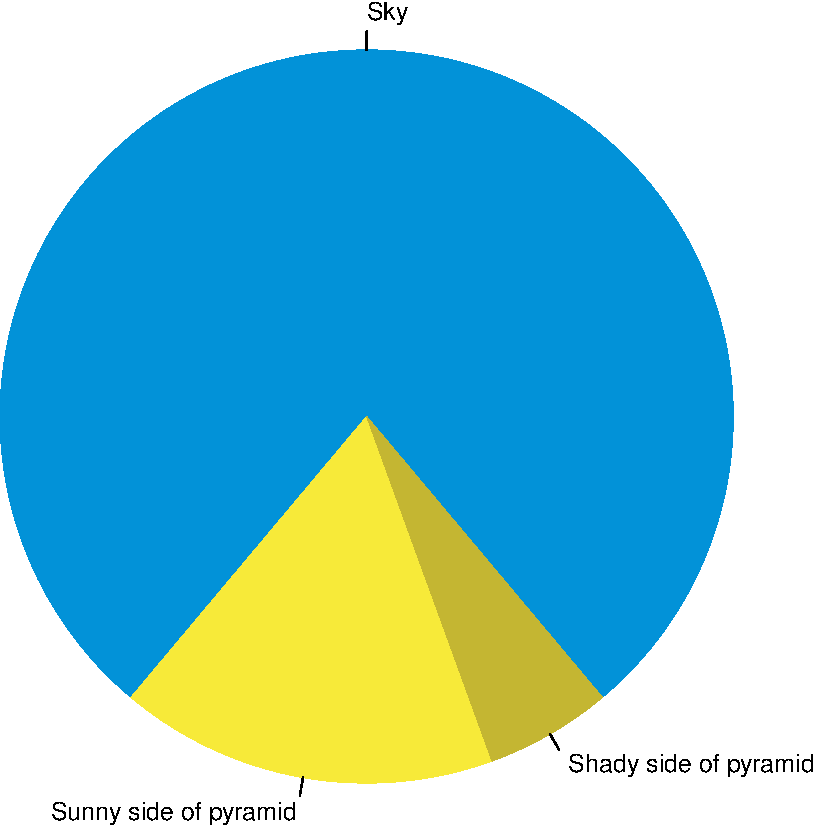
\includegraphics[width=1\linewidth]{Rmarkdown_files/figure-latex/pie-1} \caption{A fancy pie chart.}\label{fig:pie}
\end{figure}

(Credit: Yihui Xie)

\hypertarget{read-in-data-files}{%
\section{Read in data files}\label{read-in-data-files}}

\begin{Shaded}
\begin{Highlighting}[]
\NormalTok{simple\_data }\OtherTok{\textless{}{-}} \FunctionTok{read.csv}\NormalTok{(}\StringTok{"https://deepbas.io/data/simple{-}1.dat"}\NormalTok{, )}
\FunctionTok{summary}\NormalTok{(simple\_data) }
\end{Highlighting}
\end{Shaded}

\begin{verbatim}
   initials            state                age      
 Length:3           Length:3           Min.   :45.0  
 Class :character   Class :character   1st Qu.:47.5  
 Mode  :character   Mode  :character   Median :50.0  
                                       Mean   :52.0  
                                       3rd Qu.:55.5  
                                       Max.   :61.0  
     time          
 Length:3          
 Class :character  
 Mode  :character  
                   
                   
                   
\end{verbatim}

\begin{Shaded}
\begin{Highlighting}[]
\NormalTok{knitr}\SpecialCharTok{::}\FunctionTok{kable}\NormalTok{(simple\_data)}
\end{Highlighting}
\end{Shaded}

\begin{tabular}{l|l|r|l}
\hline
initials & state & age & time\\
\hline
vib & MA & 61 & 6:01\\
\hline
adc & TX & 45 & 5:45\\
\hline
kme & CT & 50 & 4:19\\
\hline
\end{tabular}

\hypertarget{hide-the-code}{%
\section{Hide the code}\label{hide-the-code}}

If we enter the \texttt{echo\ =\ FALSE} option in the R chunk (see the .Rmd file). This prevents the R code from being printed to your document; you just see the results.

\begin{tabular}{l|l|r|l}
\hline
initials & state & age & time\\
\hline
vib & MA & 61 & 6:01\\
\hline
adc & TX & 45 & 5:45\\
\hline
kme & CT & 50 & 4:19\\
\hline
\end{tabular}

  \bibliography{book.bib,packages.bib}

\end{document}
